\documentclass[english]{article}
\usepackage[latin9]{inputenc}
\usepackage{graphicx}
\usepackage{babel}

\usepackage{verbatim}
\usepackage{array}
\usepackage{bbm}
\usepackage{amsthm,amssymb,amsbsy,amsmath,amsfonts,amssymb,amscd,amstext}
\usepackage{dsfont}
\usepackage[top=2.5cm, bottom=2.5cm, left=3cm , right=3cm]{geometry}

\title{Statistical modeling and its applications Exam} %\\ \vspace{\baselineskip} %\null \\
%\Large{Processus gaussiens et mod�les de krigeage}}
\author{Mines St-Etienne -- 21st January 2015}
\date{\small No document allowed except an A4 sheet with hand written remarks from your own hand}

\begin{document}

\maketitle
\vspace{-5mm}

\subsection*{Exercise 1 (5 pts)}

We consider the function $f(x_{1},x_{2})=e^{x_{1}}\times x_{2}$.
The aim is to perform a global sensitivity analysis of $f(X_{1},X_{2})$
when $X_{1}$, $X_{2}$ are random variables following the uniform
distribution on $[-1/2,1/2]$.
\begin{enumerate}
\item {[}0.5 pt{]} Show that $E(X_{2})=0$. We denote by $m_{1}:=E(e^{X_{1}})$
(do not compute it).
\item {[}2 pts{]} Derive the Sobol-Hoeffding decomposition of $f(X_{1},X_{2})$.
\item {[}2,5 pts{]} We denote $v_{1}=\text{var}\left(e^{X_{1}}\right)$,
$v_{2}=\text{var}(X_{2})$. (Again: do not compute them).

\begin{enumerate}
\item Express the variance $D$ of $f(X_{1},X_{2})$ as a function of $m_{1},v_{1}$
and $v_{2}$. 
\item Deduce from Question 2 that the Sobol indices of the main effects
are given by: $S_{1}=0$, $S_{2}=\frac{m_{1}^{2}}{m_{1}^{2}+v_{1}}$. 
\item Deduce, with a simple argument, the expression of the Sobol index
of the interaction, $S_{1,2}$.
\end{enumerate}
\end{enumerate}

\subsection*{Exercise 2 (3 pts)}

We consider a metamodel depending on 8 input variables $X_{1},...,X_{8}$.
In the figure below, we show the result of a global sensitivity analysis
on it.
\begin{enumerate}
\item {[}1 pt{]} Interpret the results: What are the most influential input
variables, the inactive ones? Is it true that there is no interaction
between $X_{2}$ and $X_{4}$ ?
\item {[}2 pts{]} Explain how you can draw the main effect $x_{2}\mapsto\mu_{2}(x_{2})$
from $N$ simulations of $X_{1},...,X_{8}$? Make a figure.
\end{enumerate}
\begin{center}
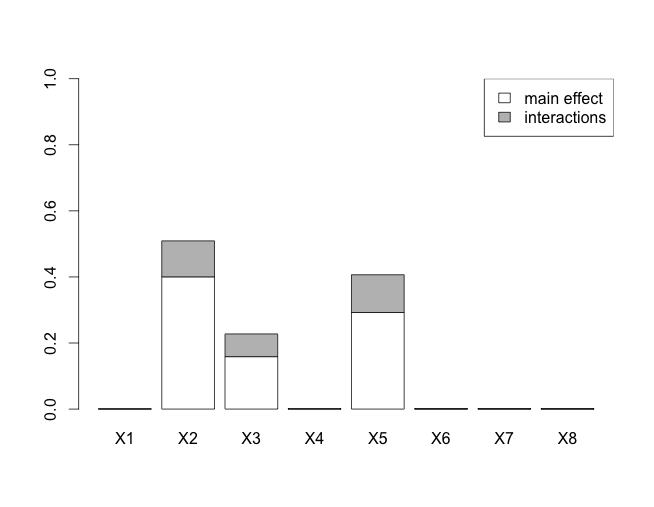
\includegraphics[width=0.8\columnwidth,height=8cm]{figures/SA_figure}
\end{center}

\newpage
\subsection*{Exercise 3 (5 pts)}
\paragraph{}
We are interested in two Gaussian process regression models based on 9 observations of a 2-dimensional function (see below). The only difference between the models is in the choice of the kernel parameters. A test set of 36 points is introduced to asses the models quality. The $Q_2$ criteria of $m_1$ and $m_2$ are respectively 0.43 and 0.69.
 %For each one, specify if your kernel is stationnary or not.
\begin{center}
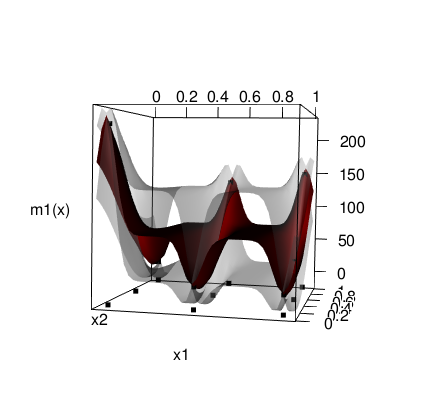
\includegraphics[width=0.5\columnwidth]{figures/model1} 
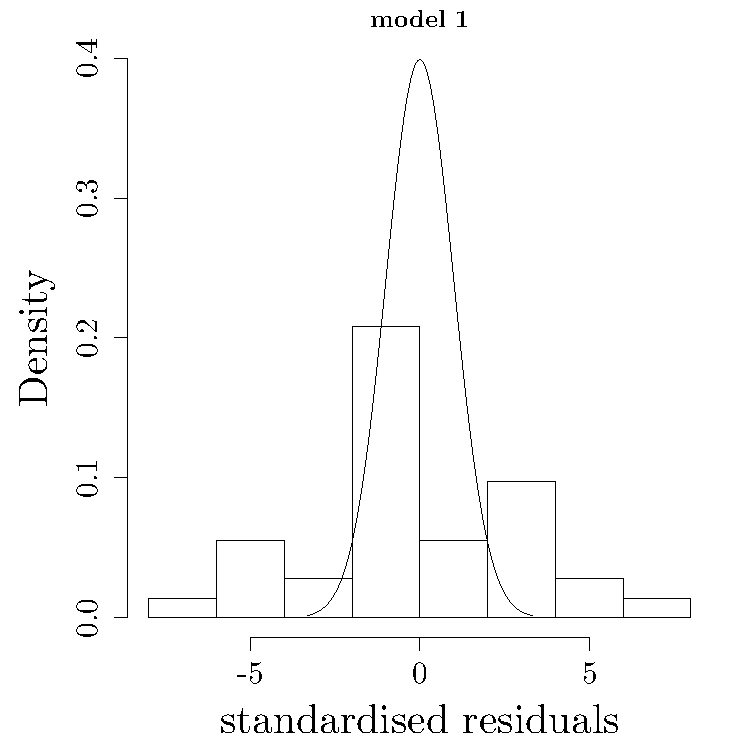
\includegraphics[width=0.4\columnwidth]{figures/res_1} \\
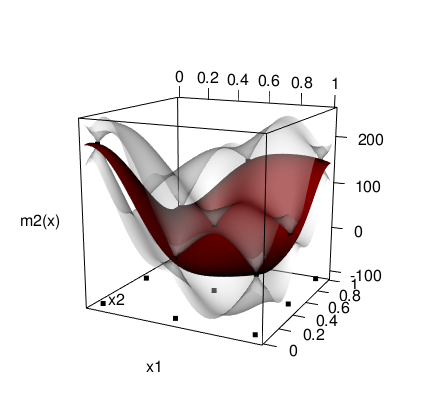
\includegraphics[width=0.5\columnwidth]{figures/model2} 
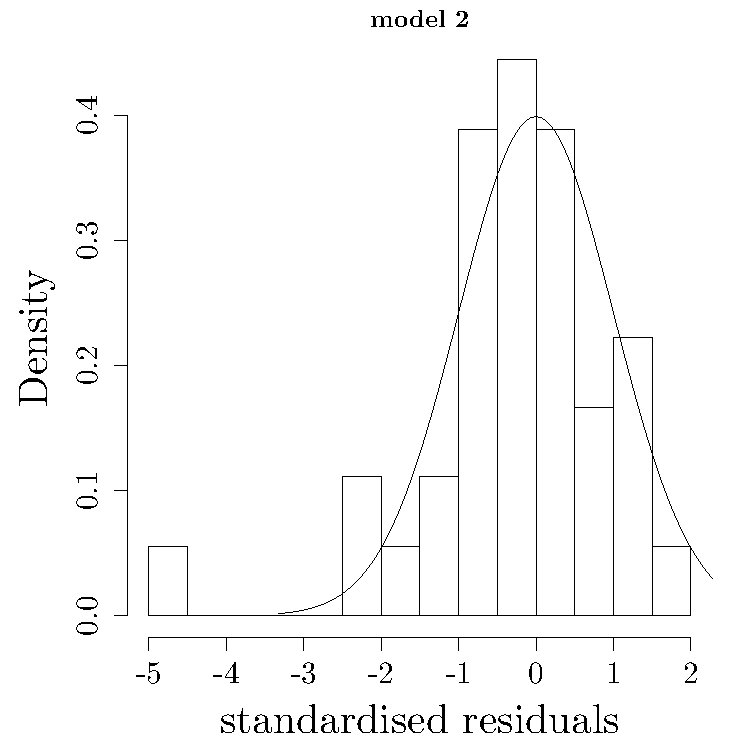
\includegraphics[width=0.4\columnwidth]{figures/res_2} \\
\end{center}

\begin{enumerate}
\item {[}1 pt{]} Give the name and expression of a kernel that may have been used.
\item {[}0.5 pt{]} For one model, the lengthscales are $(\theta_1,\theta_2)=(0.05,0.5)$ and for the other they are $(\theta_1,\theta_2)=(0.25,0.25)$. Find which is which and justify your answer.
\item {[}1.5 pt{]} How are the standardised residuals computed?
\item {[}1 pts{]} Which model seems to be the best ? Justify your answer.
\item {[}1 pt{]} Is there a trend in the models? If yes, is it possible to say if it is known or if it has been estimated?
\end{enumerate}

\subsection*{Exercise 4 (2 pts)}
\paragraph{}
Suggest a kernel (or a combination of usual kernels) for the following centred Gaussian process samples: %For each one, specify if your kernel is stationnary or not.
\begin{center}
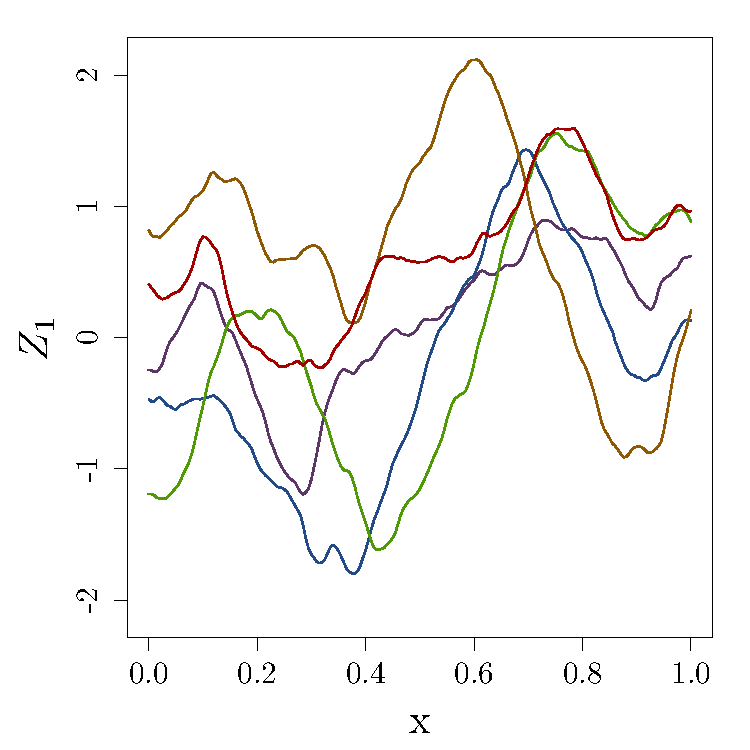
\includegraphics[width=0.33\columnwidth]{figures/traj_1} \qquad
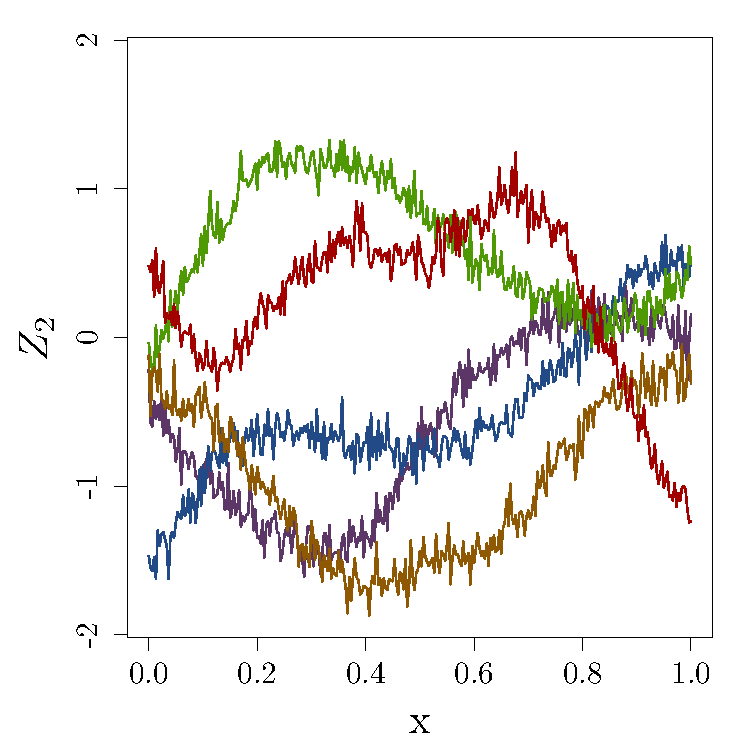
\includegraphics[width=0.33\columnwidth]{figures/traj_2} \\
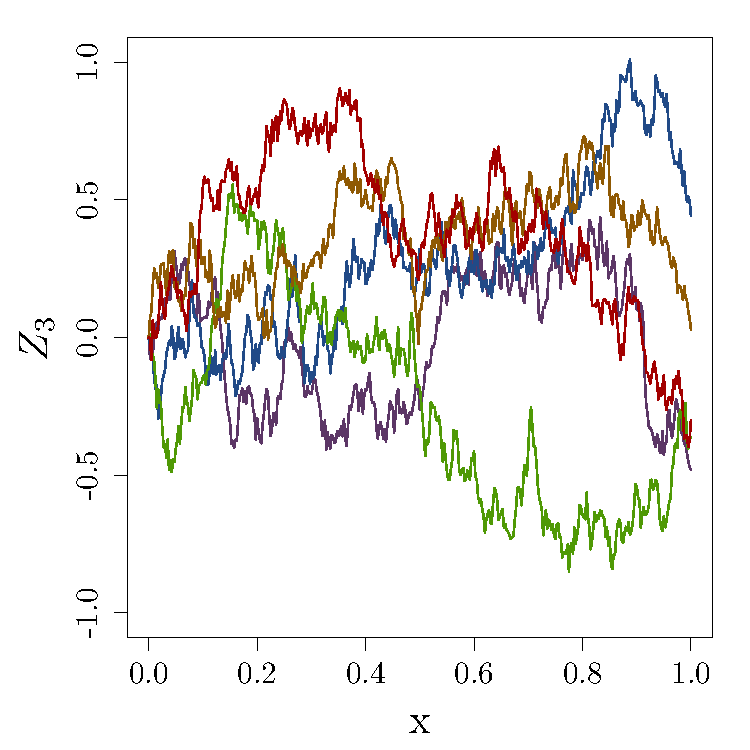
\includegraphics[width=0.33\columnwidth]{figures/traj_3} \qquad
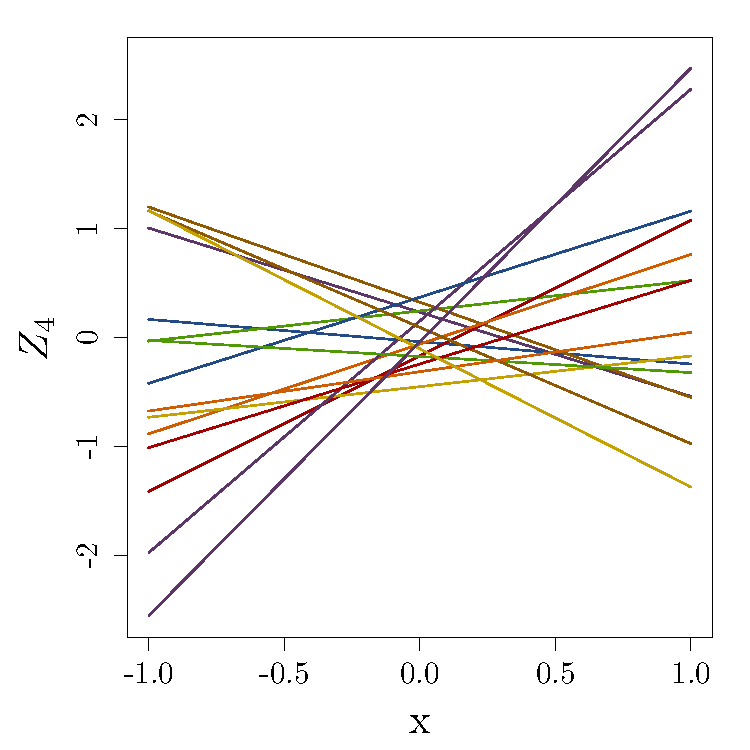
\includegraphics[width=0.33\columnwidth]{figures/traj_4} \\
\end{center}

\subsection*{Exercise 5 (3 pts)}
\paragraph{}
ANOVA kernels over $\mathds{R}^d \times \mathds{R}^d$ are kernels of the form: $\displaystyle k_{anova}(x,y) = \sigma^2 \prod_{i=1}^d (1 + k_i(x_i,y_i)) $, where the $k_i$ can be any kernel over $\mathds{R} \times \mathds{R}$.

\begin{enumerate}
\item {[}1 pt{]} Prove that $k_{anova}$ is a valid covariance function.
\item {[}1 pt{]} Write down the expression of a Gaussian process regression model based on $k_{anova}$ and show that it can be seen as the sum of $2^d$ submodels. Show that the submodels can be interpreted as a conditional Gaussian process.
\item {[}1 pt{]} Give a condition on the $k_{i}$ such that the submodel mean predictors correspond to the terms of the Sobol-Hoeffding decomposition of the mean predictor based on $k_{anova}$.
\end{enumerate}

\subsection*{Exercise 6 (2 pts)}
\paragraph{}
Let $\mathcal{H}$ be a RKHS of functions over $[0,1]$ such that the derivative evaluation in 0 : $L: f \mapsto f'(0)$ is continuous.
% \begin{equation*}
%  	\begin{split}
%  		L: \mathcal{H} & \longrightarrow \mathds{R} \\
%  		f & \longmapsto \frac{\mathrm{d} f}{\mathrm{d} x}(0)
%  	\end{split}
%  \end{equation*} 
%  is continuous.

\begin{enumerate}
\item {[}1 pt{]} Show that the Riesz theorem applies and compute the representer of $L$.
\item {[}1 pt{]} What is the reproducing kernel of the subspace $\mathcal{H}_0 = \{f \in \mathcal{H} \text{ such that }\frac{\mathrm{d} f}{\mathrm{d} x}(0)=0 \}$?
\end{enumerate}

\end{document}
























\subsection*{Exercise 1 (2014 exam)}
\paragraph{}
The graphs bellow show samples of centred Gaussian process. What kernel may have been used to generate these figures? Justify briefly your answer.
\begin{figure}[!ht]%
\begin{center}
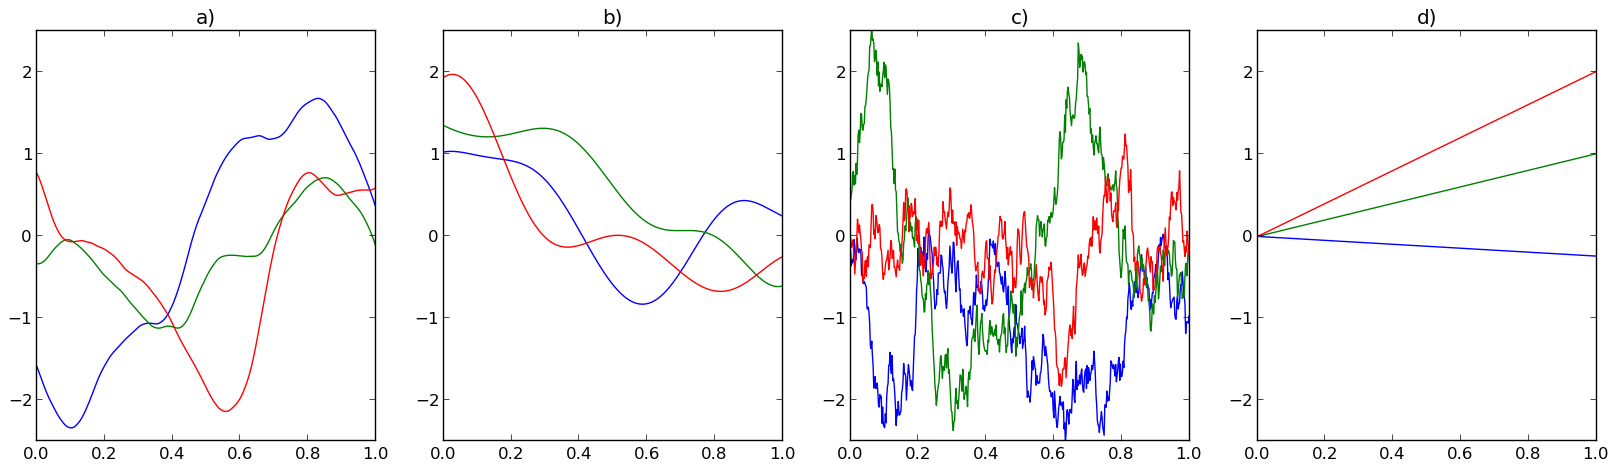
\includegraphics[width=\textwidth]{python/Ex1}
\end{center}
\end{figure}

%%%%%%%%%%%%%%%%%%%%%%%%%%%%%%%%%%%%%%%%%%%%%%%%%%%%%%%%%%%%%%%%%%%%%%%%%%%%%%%%
\subsection*{Exercise 2 (2014 exam)}
For the four models bellow, indicate:
\begin{itemize}
	\item the type of trend that is considered
	\item if the trend is known or estimated
	\item the kernel used
	\item if there is observation noise
\end{itemize}

\begin{figure}[!ht]%
\begin{center}
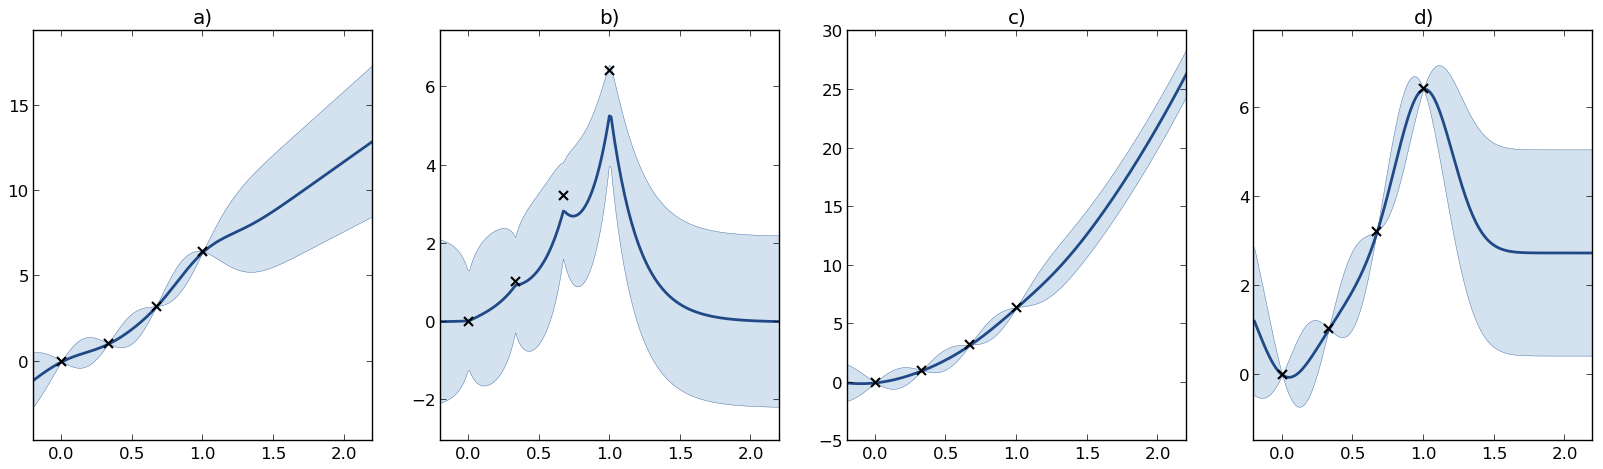
\includegraphics[width=\textwidth]{python/Ex2}
\end{center}
\end{figure}
Suggest a model that would be suited to the data at hand.

%%%%%%%%%%%%%%%%%%%%%%%%%%%%%%%%%%%%%%%%%%%%%%%%%%%%%%%%%%%%%%%%%%%%%%%%%%%%%%%%
\subsection*{Exercise 3 An alternative to ordinary kriging}
An alternative to kriging model with trend is to consider sums of kernels where some of the kernels correspond either to the space generated by basis functions or to spaces of low frequency functions. Let $X$ be a $\mathcal{N}(0,s^2)$ random variable and let $Z_1$ be the random process defined by $Z_1(x) = 1 \times X$.

\paragraph{1.} Prove that $Z_1$ is a Gaussian process. Give the expressions of it's mean $m_1$ and covariance $k_1$. 

\paragraph{2.} What happen if we try to build a Gaussian process regression model based on $Z_1$.

\paragraph{3.} Let $Z$ be a centered Gaussian process with kernel $k_Z$. We define a new GP $Y(x) = Z(x) + Z_1(x)$ where $Z$ and $Z_1$ are taken independently. What is the covariance of $Y$ ? 

\paragraph{4.} Give the expression of the Gaussian process model based on $Y$. Show that the best predictor can be written
\begin{equation*}
	m(x) = \frac{\mathbf{1}^t K^{-1} F}{1/s^2 + \mathbf{1}^t K^{-1} \mathbf{1}} + k(x,X) K^{-1} \left( F - \mathbf{1} \frac{\mathbf{1}^t K^{-1} F}{1/s^2 + \mathbf{1}^t K^{-1} \mathbf{1}} \right)
\end{equation*}
where $K = k(X,X)$. The Woodbury matrix identity will be useful to answer this question:
\begin{equation*}
	(K + UCV)^{-1} = K^{-1} - K^{-1} U (C^{-1} + V K^{-1} U)^{-1} V K^{-1}
\end{equation*}
where $K$ is a $n \times n$ invertible matrix, $U$ and $V^t$ are $n \times p$ and $C$ is $p \times p$.

\paragraph{5.} What is the conditional distributions when we predict far away from the observations?

\paragraph{6.} What is the conditional distributions when $s^2 \rightarrow + \infty$?

\paragraph{7.} Can the previous questions be adapted to build a kernel based alternative to universal kriging.

\paragraph{8.} In a similar fashion, what would be the meaning of a GPR model based on sum of squared exponential kernels $k(x,y;\sigma^2 = 1e3, \theta=20) + k(x,y;\sigma^2 = 1, \theta=1)$?

%%%%%%%%%%%%%%%%%%%%%%%%%%%%%%%%%%%%%%%%%%%%%%%%%%%%%%%%%%%%%%%%%%%%%%%%%%%%%%%%
\subsection*{Exercise 4 : GPR and linear regression}
Let $H$ be a function basis (such as $H(x)=(1,x,x^2)$) and $Z$ be a centred GP with kernel $k(x,y) = \sigma^2 H(x)H(y)^t$. 

\paragraph{1.}
How would you simulate sample paths from $Z$?

\paragraph{2.}
Given some observations $F$ with noise $\mathcal{N}(0,\tau^2)$, what would be the expression of a GPR model?

\paragraph{}
The definition of the pseudio inverse of a matrix is:
\begin{equation*}
	A^\dagger = \lim_{\delta \rightarrow 0} A^t (A A^t + \delta Id)^{-1} = \lim_{\delta \rightarrow 0} (A^t A + \delta Id)^{-1} A.
\end{equation*}
Furthermore, when $A^tA$ is invertible, we have $A^\dagger = (A^t A)^{-1} A$.

\paragraph{3.}
Using the above property, write down the expression of the best predictor when $\tau^2 / \sigma^2$ tends to zero. What can you recognize?


\end{document} 
